\documentclass[11pt]{article}

% Language setting
% Replace `english' with e.g. `spanish' to change the document language
\usepackage[english]{babel}

% Set page size and margins
% Replace `letterpaper' with`a4paper' for UK/EU standard size
\usepackage[a4paper,top=1.5cm,bottom=1.5cm,left=1.5cm,right=1.5cm,marginparwidth=1.75cm]{geometry}

% Useful packages
\usepackage{amsmath}
\usepackage{graphicx}
\usepackage[colorlinks=true, allcolors=blue]{hyperref}
\usepackage{setspace}
\usepackage[font=small,labelfont=bf]{caption}
\usepackage{titling}

\setlength{\droptitle}{-5em}
\title{IVR Coursework 1 Report}
\author{Hantao Zhong(s1904845), Zhijun Pan(s1969962)}

\begin{document}

\singlespacing  % Set line spacing to 1 from here on

\maketitle

\section{Work Separation}

In this coursework, Hantao worked on the Vision part (2.1 and 2.2) while Zhijun worked on the Control part (3.1 and 3.2). During the process, we had discussions on each other's parts and envisioned ideas and solutions together. GitHub: https://github.com/MrTooOldDriver/UoE-IVR-Coursework.git

\section{Robot Vision}

\subsection{Joint state estimation - I}

\subsubsection{Algorithm Description}

The algorithm consists of two steps. The first is to use two images from camera1 and camera2 to estimate all sphere coordinates in 3D space using blob detection. The second is using geometry vector info to find joint angles.

The blob detection algorithm interprets each image's colour sphere's coordinate. We first use the OpenCV inRange function for each colour of joints to select the sphere colour region and load it as a mask. Then using dilate function to expand and smooth the mask and, after that, use the mask's moment to find the middle point of our mask as our coordinate of a sphere.

Then we could combine spheres coordinates from camera1 and camera2 to reconstruct the 3D coordinate of each sphere. The 3D coordinate $[X,Y,Z]$ where X = - X offset between reference sphere and target sphere in camera2,  Y= - X offset between reference sphere and target sphere in camera1 and Z = average Y offset between reference sphere and target sphere in both cameras. In practice, we use the yellow sphere as our reference sphere because the resulting coordinate will be the vector from the yellow sphere. This could reduce error in practice when using the green sphere as the centre of the world since we use lots of yellow sphere vectors for calculation.

After obtaining every sphere's 3D coordinate, we could obtain the vector $\Vec{Yellow Blue}$. We could find out joint2 by calculating the angle between the z-axis($[0,0,1]$) and vector $\Vec{Yellow Blue}$ projection on the xz plane. ($Vector=[x,y,z]$ projection on xz plane $= [x, 0, z]$). After obtaining joint2 we could calculate the new xz plane projection after joint2 rotations (new projection on xz plane $= [sin(joint2), 0, cos(joint2)]$). Then calculate the angle between the new projection plane and the vector $\Vec{Yellow Blue}$, we get joint3 angle.

For finding joint4, we first find the vector $\Vec{Yellow Red}$, then $\Vec{Yellow Red} - \Vec{Yellow Blue} = \Vec{Red Blue}$. By calculating the angle between $\Vec{Red Blue}$ and $\Vec{Yellow Blue}$, we get joint4. Since the blue joint only could move around one axis.

If any mask moment M['m00'] is zero, then some spheres are not visible. Hence the algorithm will use other spheres locations as no visible sphere location. (e.g. when the blue sphere is invisible, it will use yellow sphere location since it is the only possible situation)

\subsubsection{Plots}

\begin{center}
\begin{minipage}{0.33\linewidth}
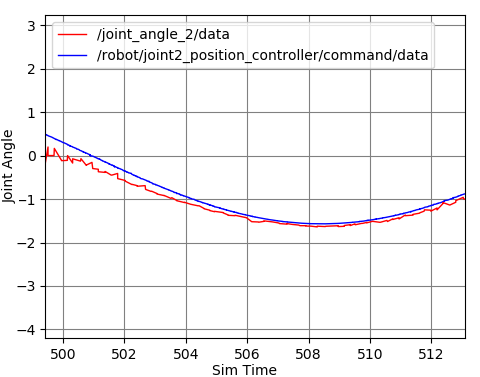
\includegraphics[width=\linewidth]{fig_with_axisname/2.1-joint2.png}
\captionof{figure}{Joint2 result}
\end{minipage}%
\hfill
\begin{minipage}{0.33\linewidth}
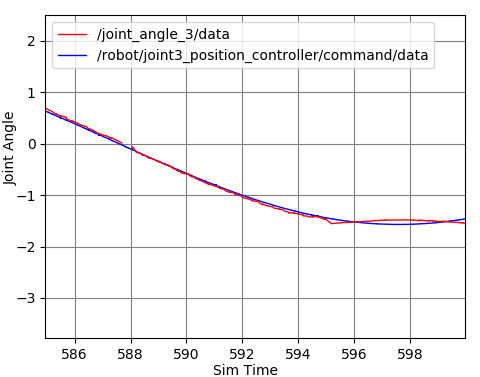
\includegraphics[width=\linewidth]{fig_with_axisname/2.1-joint3.png}
\captionof{figure}{Joint3 result}
\end{minipage}
\hfill
\begin{minipage}{0.33\linewidth}
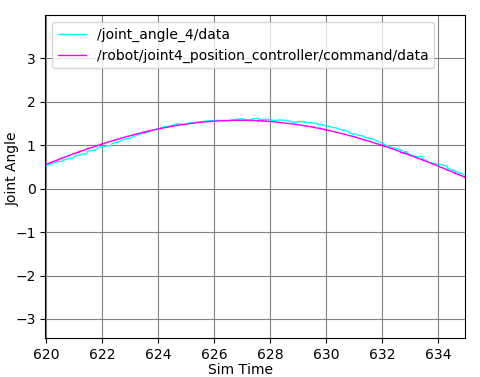
\includegraphics[width=\linewidth]{fig_with_axisname/2.1-joint4.png}
\captionof{figure}{Joint4 result}
\end{minipage}%
\end{center}



\subsubsection{Observations and Analysis}

For joint2, sometimes the estimated value suddenly moves up or down with a huge value(pi or -pi). This is because the sphere partially blocks another sphere, and the sphere detection accuracy will decrease as the visible area reduces as it can't see the whole sphere area. Hence using a moment to estimate visible area will start to become inaccurate.

For joint3, the estimated value is very close to the actual value for all the time. But since we use joint2 to calculate the xz plane projection, our joint2 is sometimes inaccurate, which will affect our joint3 result. This is why we see some peaks and bottom in our result.

For joint4, our algorithm could detect the angle of joint4 very well but can't determine the signed angle due to the nature of calculating the vector angle. It is hard to decide on the angle sign because joint2 and joint3 are constantly changing. The change of joint2 and joint3 will change the reference frame of joint4. Hence, we can't determine whether joint4 moving is positive or negative.

\subsection{Joint state estimation - II}

\subsubsection{Algorithm Description}

For this section, the robot only has joint1 3 4 is movable. First, we still use the same method in 2.1 to find each sphere's coordinate in 3D space via two camera images. Then using coordinate to find geometry information of each joint(e.g. vector from yellow sphere to a blue sphere $\Vec{Yellow Blue}$). For joint1, we calculate and use the angle between the positive y-axis and vector $\Vec{Yellow Blue}$ as our joint1 angle and the angle between the positive z-axis and vector $\Vec{Yellow Blue}$ as our joint2 angle. We use vector $\Vec{Yellow Blue}$ to calculate joint1 is because the movement around the z-axis is not directly visible by our camera. We have to interpret vector $\Vec{Yellow Blue}$'s direction to blue corresponding with z-axis. But this introduces an issue since joint3 is also moving between $\pi/2$  and $-\pi/2$. The angle between the positive y-axis and vector $\Vec{Yellow Blue}$ is not the same when joint3 moves in positive angle and negative angle. Hence we can't ensure which angle is the actual angle if we don't know about joint3. However, joint3 also has similar issues since we need to joint1 angle to determine whatever joint3 is positive or negative. Hence the signs of joint1 and joint3 depend on each other. Just like a chicken or the egg question. Therefore we can't always determine the true angles of joint1 and joint3.

For joint4, we still use the same algorithm as 2.1, using the vector angle formula to calculate the angle between vector $\Vec{Yellow Blue}$ and vector $\Vec{Blue Red}$. The signed angle problem remains in the algorithm.

\subsubsection{Plots}

\begin{center}
\begin{minipage}{0.33\linewidth}
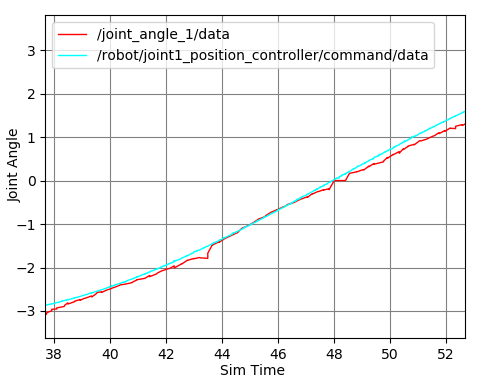
\includegraphics[width=\linewidth]{fig_with_axisname/2.2-joint1.png}
\captionof{figure}{Joint1 result}
\end{minipage}%
\hfill
\begin{minipage}{0.33\linewidth}
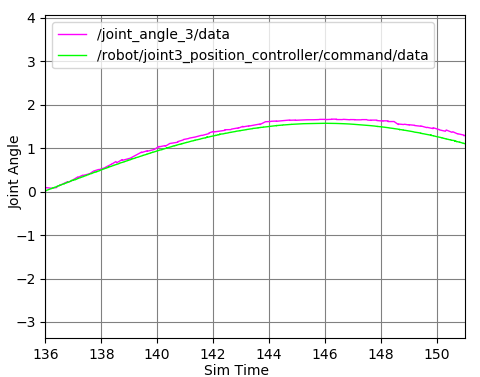
\includegraphics[width=\linewidth]{fig_with_axisname/2.2-joint3.png}
\captionof{figure}{Joint3 result}
\end{minipage}
\hfill
\begin{minipage}{0.33\linewidth}
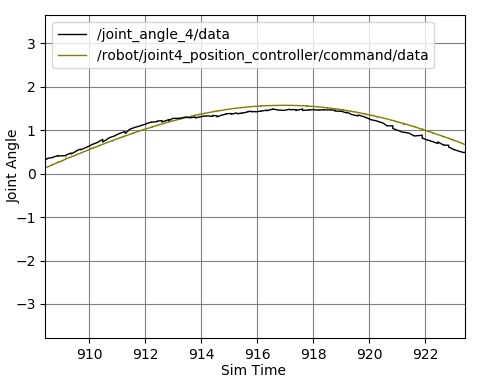
\includegraphics[width=\linewidth]{fig_with_axisname/2.2-joint4.png}
\captionof{figure}{Joint4 result}
\end{minipage}
\end{center}

\section{Robot Control}

\subsection{Forward Kinematics}

\subsubsection{The Homogeneous Transformation}

The homogeneous transformation matrix is:
\begin{equation}
\begin{split}
    H=\begin{bmatrix} R_{n}^{0} & O_{n}^{0} \\ 0 & 1 \end{bmatrix}, A_{i}=\begin{bmatrix} R_{i}^{i-1} & O_{i}^{i-1} \\ 0 & 1 \end{bmatrix}
\end{split}
\end{equation}
where $R$ is a 3x3 matrix representing rotation and $O$ is a 3d vector representing coordinates which in this represents the displacements (translations) between joints. The final transformation matrix $H$ is a multiplication of transformation matrices $A$ on each joint angle where $H=A_{1}(q_{1})...A_{n}(q_{n})$. Hence, for the transformation from the origin to joint 1, 3, 4 and the end-effector, the final matrix $H$ is (the result of $H$ is way too long so we omitted it here):
\begin{equation}
\begin{split}
    & H=A_{1}A_{3}A_{4}A_{end}
    =\begin{pmatrix}cos\left(\theta _{1}\right)&-sin\left(\theta _{1}\right)&0&0\\ \:\:\:\:\:sin\left(\theta _{1}\right)&cos\left(\theta _{1}\right)&0&0\\ \:\:\:\:\:0&0&1&0\\ \:\:\:\:\:0&0&0&1\end{pmatrix}
    \begin{pmatrix}1&0&0&0\\ \:\:\:\:0&cos\left(\theta _{3}\right)&-sin\left(\theta _{3}\right)&0\\ \:\:\:\:\:\:0&sin\left(\theta _{3}\right)&cos\left(\theta _{3}\right)&4\\ \:\:\:\:\:\:0&0&0&1\end{pmatrix} \\ 
    & \begin{pmatrix}cos\left(\theta _{4}\right)&0&sin\left(\theta _{4}\right)&0\\ \:\:\:0&1&0&0\\ \:\:\:-sin\left(\theta _{4}\right)&0&cos\left(\theta _{4}\right)&3.2\\ \:\:\:0&0&0&1\end{pmatrix} \begin{pmatrix}1&0&0&0\\ \:0&1&0&0\\ \:0&0&1&2.8\\ \:0&0&0&1\end{pmatrix} \\
\end{split}
\end{equation}
To only get the last column of $H$ (which is $\begin{pmatrix}O_{n}^{0}\\ 1\end{pmatrix}$), we multiply $H$ by the vector $(0 \: 0 \: 0 \: 1)$:
\begin{equation}
\begin{split}
    & \begin{pmatrix}O_{n}^{0}\\ 1\end{pmatrix} = H\begin{pmatrix}0\\ 0\\ 0\\ 1\end{pmatrix}
    = \begin{pmatrix}3.2\sin \left(\theta _{1}\right)\sin \left(\theta _{3}\right)+2.8\left(\cos \left(\theta _{1}\right)\sin \left(\theta _{4}\right)+\sin \left(\theta _{1}\right)\sin \left(\theta _{3}\right)\cos \left(\theta _{4}\right)\right)\\ 2.8\left(\sin \left(\theta _{1}\right)\sin \left(\theta _{4}\right)-\cos \left(\theta _{1}\right)\sin \left(\theta _{3}\right)\cos \left(\theta _{4}\right)\right)-3.2\cos \left(\theta _{1}\right)\sin \left(\theta _{3}\right)\\ 2.8\cos \left(\theta _{3}\right)\cos \left(\theta _{4}\right)+3.2\cos \left(\theta _{3}\right)+4\\ 1\end{pmatrix}
\end{split}
\end{equation}
where $O_{n}^{0}$ are the end-effector's position coordinates.

\subsubsection{The Result of Forward Kinematics Calculation}

The calculation of homogeneous transformation matrix $H$ is shown in the last section, and the 3-d vector $O_{n}^{0}$ is the final location of the end-effector. Hence, the forward kinematics in this case is:
\begin{equation}
\begin{split}
k_{e}=K(\mathbf{q})=O_{n}^{0}=\begin{pmatrix}3.2\sin \left(\theta _{1}\right)\sin \left(\theta _{3}\right)+2.8\left(\cos \left(\theta _{1}\right)\sin \left(\theta _{4}\right)+\sin \left(\theta _{1}\right)\sin \left(\theta _{3}\right)\cos \left(\theta _{4}\right)\right)\\ 2.8\left(\sin \left(\theta _{1}\right)\sin \left(\theta _{4}\right)-\cos \left(\theta _{1}\right)\sin \left(\theta _{3}\right)\cos \left(\theta _{4}\right)\right)-3.2\cos \left(\theta _{1}\right)\sin \left(\theta _{3}\right)\\ 2.8\cos \left(\theta _{3}\right)\cos \left(\theta _{4}\right)+3.2\cos \left(\theta _{3}\right)+4\end{pmatrix}
\end{split}
\end{equation}
where $k_{e}$ is the coordinates of the end-effector and $\mathbf{q}=\begin{pmatrix}\theta_{1}\\ \theta_{2}\\ \theta_{3}\\ \theta_{4}\end{pmatrix}$.

\subsubsection{Verifying the Results of Forward Kinematics Calculation}

A table comparing the end-effector positions via FK calculation to detection using images:
\begin{center} 
\begin{tabular}{ | c | c | c | c | }
\hline
\textbackslash & Joint angles [$\theta_{1}$, $\theta_{3}$, $\theta_{4}$] & FK calculation result [$x, y, z$] & Detection from image [$x, y, z$] \\ 
\hline 
1 & [1.0, 1.0, 1.0] & [4.610, -0.160, 6.546] & [4.650, -0.035, 5.981]  \\
2 & [1.3, 1.5, 0.8] & [5.487, 0.561, 4.364] & [5.183, 0.852, 3.603]  \\
3 & [1.6, 0.8, 2.0] & [1.384, 2.587, 5.417] & [1.846, 3.195, 5.626]  \\
4 & [2.5, 1.1, 0.4] & [2.208, 4.778, 6.621] & [1.881, 5.254, 5.999]  \\
5 & [1.1, 2.0, 1.2] & [4.599, 0.587, 2.246] & [4.828, 0.816, 3.053]  \\
6 & [1.9, 0.5, 0.6] & [1.989, 2.350, 8.836] & [1.881, 2.520, 8.182]  \\
7 & [3.0, 2.8, 2.5] & [-1.613, 0.553, 3.098] & [-1.775, -0.071, 3.851]  \\
8 & [2.8, 2.0, 1.0] & [-0.784, 4.827, 2.038] & [-0.461, 4.828, 3.709]  \\
9 & [0.8, 0.8, 0.8] & [4.049, -1.133, 7.588] & [4.366, -1.242, 7.188]  \\
10 & [0.6, 0.7, 0.9] & [3.607, -1.388, 7.778] & [3.976, -1.526, 7.401]  \\
\hline 
\end{tabular} 
\end{center}
Comments: From the table, we can see that the end-effector positions calculated via FK is always close to the positions via detection using images. As the result of FK calculation is definite, the difference only comes the errors in detection. By the data in the table plus verification by looking at the output images, the FK calculations can be confirmed correct and accurate.

\subsection{Inverse Kinematics}

\subsubsection{Calculating Joint Angles}

In order to get the end-effector to a target position, we calculate the joint angles required to achieve the effect. We have $\mathbf{\dot{x}}=J(\mathbf{q})\mathbf{\dot{q}}$ where $J(\mathbf{q})$ is the Jacobian matrix, $\mathbf{\dot{x}}$ is the target position, $\mathbf{q}$ is the current joint angles and $\mathbf{\dot{q}}$ is the desired joint angles. Hence $\mathbf{\dot{q}}=J^{-1}\mathbf{\dot{x}}$ where $J^{-1}$ is the inverse of Jacobian matrix.

\subsubsection{Calculating Jacobian and Its Inverse}

Jacobian matrix is a partial derivative of the FK equation $K(\mathbf{q})$ with respect to change of time $dt$. So (the resultant $J$ is too long so separated into columns):
\begin{equation}
\begin{split}
& J=\frac{\partial K(\mathbf{q})}{\partial \mathbf{q}} = \\
& column \: 0: \begin{pmatrix}-2.8\sin\left(\theta_{1}\right)\sin\left(\theta_{4}\right)\:+\:2.8\sin\left(\theta_{3}\right)\cos\left(\theta_{1}\right)\cos\left(\theta_{4}\right)\:+\:3.2\sin\left(\theta_{3}\right)\cos\left(\theta_{1}\right)\\ 2.8\sin\left(\theta_{1}\right)\sin\left(\theta_{3}\right)\cos\left(\theta_{4}\right)\:+\:3.2\sin\left(\theta_{1}\right)\sin\left(\theta_{3}\right)\:+\:2.8\sin\left(\theta_{4}\right)\cos\left(\theta_{1}\right)\\ 0\end{pmatrix} \\
& column \: 1: \begin{pmatrix}2.8\sin\left(\theta_{1}\right)\cos\left(\theta_{3}\right)\cos\left(\theta_{4}\right)\:+\:3.2\sin\left(\theta_{1}\right)\cos\left(\theta_{3}\right)\\ -2.8\cos\left(\theta_{1}\right)\cos\left(\theta_{3}\right)\cos\left(\theta_{4}\right)\:-\:3.2\cos\left(\theta_{1}\right)\cos\left(\theta_{3}\right)\\ -2.8\sin\left(\theta_{3}\right)\cos\left(\theta_{4}\right)\:-\:3.2\sin\left(\theta_{3}\right)\end{pmatrix} \\
& column \: 2: \begin{pmatrix}-2.8\sin\left(\theta_{1}\right)\sin\left(\theta_{3}\right)\sin\left(\theta_{4}\right)\:+\:2.8\cos\left(\theta_{1}\right)\cos\left(\theta_{4}\right)\\ 2.8\sin\left(\theta_{1}\right)\cos\left(\theta_{4}\right)\:+\:2.8\sin\left(\theta_{3}\right)\sin\left(\theta_{4}\right)\cos\left(\theta_{1}\right)\\ -2.8\sin\left(\theta_{4}\right) \cos\left(\theta_{3}\right)\end{pmatrix} 
\end{split}
\end{equation}
As the Jacobian is not inevitable in general, we calculate its pseudo-inverse: $J^{\dagger}=J^{T}(JJ^{T})^{-1}$.

\subsubsection{Executing Inverse Kinematics}

Once we have the inverse of Jacobian matrix, we can calculate the desired $q_{des}=q_{curr}+\Delta t J^{-1}\mathbf{\dot{x}}$ where $\Delta t$ is the time difference since last execution and $q_{curr}$ are the current joint angles' states. After iterations, the end-effector's position should approach the target position.

\subsubsection{Plots comparing the x, y, and z positions}

\begin{center}
\begin{minipage}{0.5\linewidth}
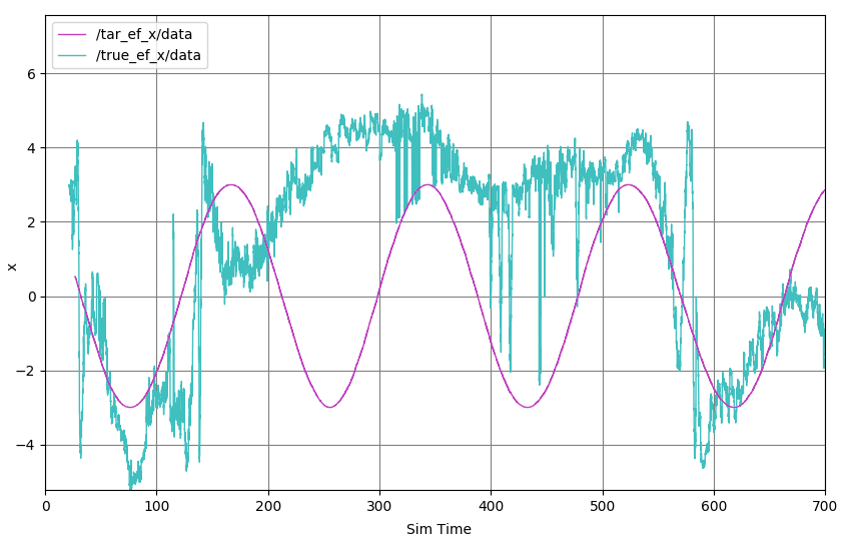
\includegraphics[width=\linewidth]{fig_with_axisname/ikx2.png}
\captionof{figure}{end-effector target vs publish on x}
\end{minipage}%
\hfill
\begin{minipage}{0.5\linewidth}
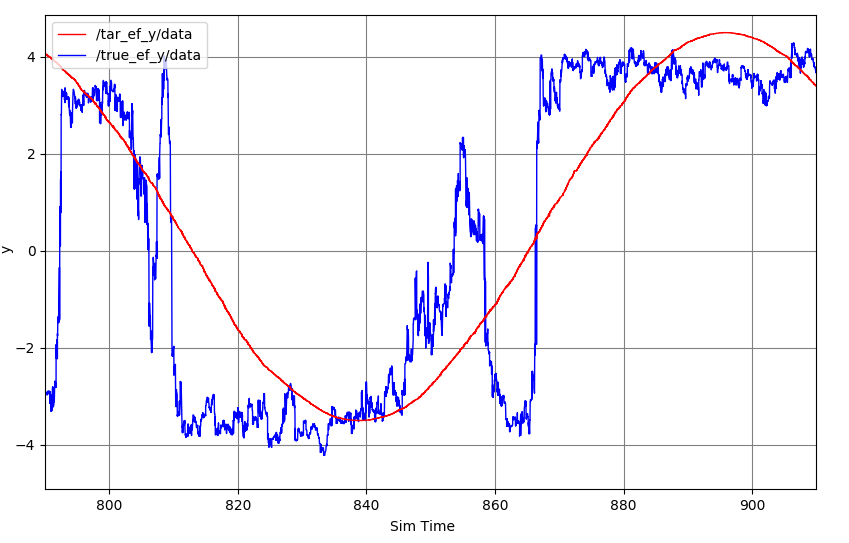
\includegraphics[width=\linewidth]{fig_with_axisname/iky2.png}
\captionof{figure}{end-effector target vs publish on y}
\end{minipage}
\end{center}

\begin{center}
\begin{minipage}{0.5\linewidth}
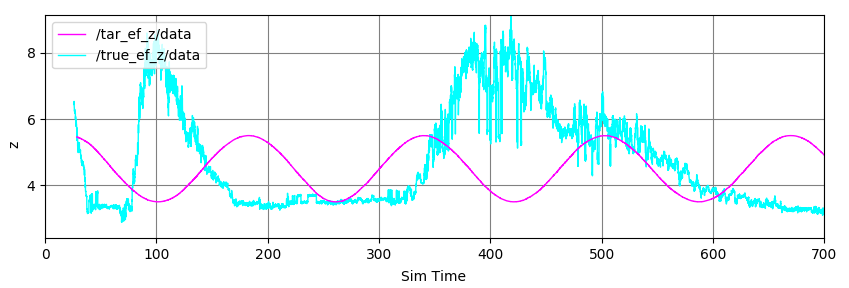
\includegraphics[width=\linewidth]{fig_with_axisname/ikz2.png}
\captionof{figure}{end-effector target vs publish on z}
\end{minipage}%
\end{center}



\end{document}